\documentclass[article,12pt]{elsarticle}
\usepackage[spanish]{babel}
\usepackage[utf8]{inputenc}
\usepackage{amssymb}
\usepackage{flushend}
\usepackage{float}
\usepackage{anysize}
\usepackage{amsmath}
\usepackage{amsfonts}
\usepackage{dcolumn}
\usepackage{amsthm}
\usepackage{caption}
\usepackage{float}
\usepackage{subfigure}
\usepackage{graphicx}
\usepackage{lmodern}
\usepackage{booktabs}
\usepackage{color}
\usepackage{longtable}
\usepackage{rotating}
\usepackage{etoolbox}
\usepackage{comment}
\usepackage{pdflscape}
\usepackage{booktabs}


\begin{document}

\begin{frontmatter}
    \title{Laboratorio de Electromagnetismo \\  Práctica  7\\ 
        Circuitos eléctricos RC}
    \author{Iván Bautista Alvarado$^1$ y Andrés López González$^1$} %Aquí va el nombre de los integrantes que participaron en el informe.
    \address{$^1$ Facultad de Ciencias, Universidad Nacional Autónoma de México, M\'exico CDMX.}


    \begin{abstract}
In electrical circuits containing resistors, it is possible to calculate an equivalent or total resistance, which is crucial for understanding current flow and voltage drops. This paper addresses the study of resistors in series and parallel configurations, as well as RC (resistor-capacitor) circuits to analyze the charging and discharging behavior of capacitors.

To validate theoretical predictions, two experimental setups were performed: one with resistors connected in series and parallel, and another involving the discharge of capacitors in an RC circuit. The tools used included a breadboard, power supply, multimeter, and oscilloscope. Resistance values were measured in various configurations, and voltage and current measurements were taken to verify Kirchhoff’s laws. In the RC circuits, different resistor-capacitor pairs were tested to calculate the time constant \( \tau \) and assess its accuracy against theoretical values.

The results show that the experimental data for series and parallel resistors agree with theoretical predictions, with minor discrepancies attributed to conductor resistance and external circuit elements. For the RC circuits, we observed the characteristic exponential decay in the capacitor's discharge curve, with experimental values of \( \tau \) closely matching theoretical calculations. These findings confirm the applicability of Kirchhoff’s laws and the exponential decay model in predicting circuit behavior, providing a practical approach for obtaining accurate measurements of circuit parameters and optimizing electronic circuit design.

\end{abstract}

    \begin{keyword}
     Electric circuits, Kirchhoff's laws, Ohm's law, RC circuit, Time constant
    \end{keyword}
\end{frontmatter}
\section*{Resumen}
En circuitos eléctricos que contienen resistencias, es posible calcular una resistencia equivalente o total, lo cual es crucial para comprender el flujo de corriente y las caídas de voltaje. Este artículo aborda el estudio de resistencias en configuraciones en serie y en paralelo, así como la de circuitos RC (resistor-capacitor) para analizar el comportamiento de carga y descarga de capacitores.

Para validar las predicciones teóricas, se realizaron dos montajes experimentales: uno con resistencias conectadas en serie y paralelo, y otro que involucró la descarga de capacitores en un circuito RC. Las herramientas utilizadas incluyeron una protoboard, fuente de alimentación, multímetro y osciloscopio. Se midieron los valores de resistencia en diversas configuraciones, y se tomaron mediciones de voltaje y corriente para verificar las leyes de Kirchhoff. En los circuitos RC, se probaron distintos pares de resistencia y capacitancia para calcular la constante de tiempo \( \tau \) y evaluar su precisión en comparación con los valores teóricos.

Los resultados muestran que los datos experimentales para resistencias en serie y en paralelo concuerdan con las predicciones teóricas, con pequeñas discrepancias atribuibles a la resistencia de los conductores y elementos externos del circuito. En el caso de los circuitos RC, se observó el característico decaimiento exponencial en la curva de descarga del capacitor, con valores experimentales de \( \tau \) que coinciden estrechamente con los cálculos teóricos. Estos hallazgos confirman la aplicabilidad de las leyes de Kirchhoff y el modelo de decaimiento exponencial en la predicción del comportamiento de los circuitos, aportando un enfoque práctico para obtener mediciones precisas de los parámetros del circuito y optimizar el diseño de circuitos electrónicos.


\noindent \textit{Palabras clave:}  Circuitos RC; Leyes de Kirchhoff; Descarga de capacitores; Resistencia equivalente; Constante de tiempo.

\section{Introducción}
Cuando tenemos circuitos eléctricos cerrados con resistencias, podemos calcular una resistencia equivalente o resistencia total.

\textbf{Resistencias en serie:}
\begin{equation}
        R_T = \sum_i R_i
    \end{equation}
\textbf{Resistencias en paralelo:}
\begin{equation}
        \frac{1}{R_T} = \sum_i \frac{1}{R_i}
    \end{equation}
Usaremos las \textbf{Leyes de Kirchhoff}, así que es importante recordar:

\textbf{Primera Ley}
Se relaciona con la conservación de la carga, pues te dice que, al estar en un circuito de varias mallas, en un nodo, la corriente que incide es igual a la corriente en la que se divide.
\begin{equation}
    \sum_i i_{inc} = \sum_j i_{div}
\end{equation}

\textbf{Segunda Ley}
Esta Ley se relaciona con la conservación de la energía, y dice que la caída de potencial en un circuito cerrado es 0.
\begin{equation}
    V_i=V_f 
\end{equation}
También es necesario recordar la \textbf{Ley de Ohm}, que nos indica una relación entre la resistencia, el votaje y la corriente eléctrica:


En un circuito RC, se tiene una fuente de voltaje conectada a una o varias resistencias, y a su vez conectada en paralelo a un capacitor. Como se muestra en la figura.
\begin{figure}[H]
    \centering
    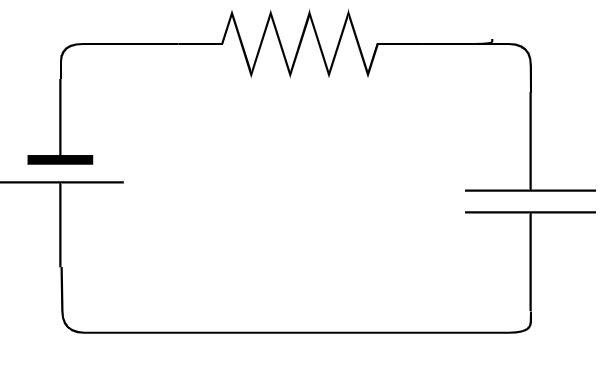
\includegraphics[width=0.5\linewidth]{CircuitoRC.jpg}
    \caption{Diagráma de un Circuito RC cuando el capacitor se carga}
\end{figure}
En este tipo de circuitos, la corriente eléctrica pasa por la resistencia y empieza a cargar al capacitor. Hasta que alcanza su carga máxima y la corriente eléctrica se "detiene".

En este punto el capacitor puede descargarse si cambiamos el circuito a uno como el de la Figura 2. Esto puede hacerse manualmente, o al activar un interruptor que permita la corriente de esta manera y desconecte a la batería.
Debido a la resistencia, la descarga del capacitor no va a ser instantanea, y va a tardar un tiempo t en descargarse.
\begin{figure}[H]
    \centering
    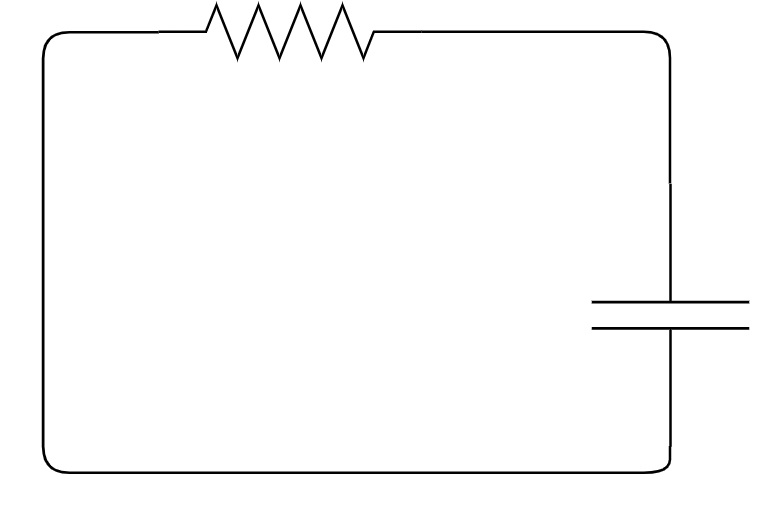
\includegraphics[width=0.4\linewidth]{CircuitoRC2.jpg}
    \caption{Diagráma de un Circuito RC cuando el capacitor se descarga}
\end{figure}
Podemos utilizar las Leyes de Kirchhoff para entender la descarga del capacitor. Considerando un circuito como el de la Figura 2. Tenemos, por segunda Ley de Kirchhoff que

\begin{align*}
    &- V_C - V_R = 0   \\
    & V_C + V_C = 0  \\
    & IR + \frac{q}{C}  = 0\\
    & \frac{dq}{dt}R - \frac{q}{C} = 0 \\
    & \frac{dq}{dt}R = \frac{q}{C}\\
    & \\
\end{align*}
Resulta en una ecuacuación diferencial para q. Si suponemos que en el tiempo t=0 el capacitor tiene una carga $q_0$. La ecuación que describe la descarga del capacitor es:
\begin{equation}
q(t) = q_0 e^{-\frac{t}{\tau}}
\end{equation}

En donde \(q(t)\) es la carga en el capacitor en el tiempo \(t\), \(q_0\) es la carga inicial del capacitor, \(\tau\) es la constante de tiempo del circuito definida como \(\tau = RC\).

La constante de tiempo \(\tau\) es un parámetro clave que caracteriza la rapidez con la que el capacitor se descarga. Físicamente, \(\tau\) representa el tiempo en el cual la carga en el capacitor se reduce a un \(36.7879\%\) de su valor inicial. Esto se puede deducir fácilmente de la ecuación, evaluando \(q(\tau)\):

\begin{equation}
q(\tau) = q_0 e^{-1} \approx 0.367879 q_0
\end{equation}

Este comportamiento es típico de sistemas que presentan decaimiento exponencial, donde la constante de tiempo define la escala temporal del proceso; la constante de tiempo \(\tau\) 
se calcula multiplicando la resistencia \(R\) del circuito en ohmios \(\Omega\) por la capacitancia \(C\) del capacitor en faradios (F):

\begin{equation}
\tau = R C
\end{equation}

En un contexto experimental, \(\tau\) se puede obtener visualmente al medir el tiempo que tarda la carga del capacitor en reducirse al $\approx$36.8\% de su valor inicial durante la fase de descarga. Esto puede observarse directamente en la gráfica \(q(t)\) vs. \(t\) obtenida con el osciloscopio, pero hemos mencionar que para obtener una buena gráfica debemos generar señales digitales (coloquialmente cuadradas) a una frecuencia dependiente de cada pareja resistencia capacitor para obtener un buen muestreo del comportamiento del capacitor. Asímismo, podemos obtenerla teóricamente observando la capacitancia y resistencia marcadas en el componente electrónico, o de forma experimental con la capacitancia medida en el capacitómetro así como la resistencia obtenida en el multímetro.

En la gráfica \(q(t)\) vs. \(t\) durante la descarga, la curva exponencial decrece rápidamente al principio, y luego de forma más lenta conforme se acerca a cero. El punto donde la curva alcanza el 36.8\% de la carga inicial \(q_0\) indica el tiempo \(\tau\). Este es un valor clave que debe ser identificado con precisión para caracterizar el circuito; nótese que para una descarga total el tiempo debe tender a infinito.

Por lo tanto, en la fase de descarga, \(\tau\) corresponde al tiempo que transcurre desde el inicio de la descarga hasta que la carga del capacitor alcanza aproximadamente un tercio de su valor inicial, lo que es visualmente identificable en la gráfica mostrada por el osciloscopio mediante una interpolación precisa de los datos registrados.
    \subsection{Hipótesis}
    \subsection{Objetivos}
        \begin{enumerate}
        \item Comparar las resistencias expermientales de circuitos con resistencias en serie y en paralelo con las teóricas.
        \item Determinar la constante de tiempo de descarga $\tau$ de un circuito RC.
    \end{enumerate}

\section{Desarrollo Experimental / Métodos}
En este repote se juntarán dos experimentos.
    \subsection{Circuitos R en serie y paralelo}
        Materiales utilizados:
        \begin{itemize}
            \item 1 Protoboard
            \item 1 Fuente de poder
            \item 2 Cables banana - banana
            \item 2 Caimanes
            \item 1 Multímetro
            \item 1 Medidor de Capacitancia
            \item 3 Resistencias de 100 $\Omega$
            \item 1 Resistencia de 60 $\Omega$
            \item 1 Resistencia de 330 $\Omega$
            \item 3 Capacitores de la misma capacitancia
            \item 3 Capacitores de distintas capacitancias
            \item 4 Cables puente
        \end{itemize}
    Para el desarrollo de este experimento, se hicieron circuitos en la Protoboard con las resistencias.

    Primero se tomaron las tres resistencias \textbf{iguales}, y se conectaron en serie.
    Se conectaron los cables banana-banana a la fuente, y con ayuda de los caimanes, se conectaron los cables banana-banana a los cables puente del circuito, para poder pasar corriente a través del circuito. De esta manera.
    Antes de encender la fuente, se midió, con el multímetro, la resistencia equivalente del circuito entero.
    Una vez encendida la fuente, se midió el voltaje que tenía cada resistencia por separado, y después el votlaje que se tenía en los extremos del circuito. Por último, se fue midiendo la corriente que pasaba por cada resistencia por individual, y luego la corriente que pasaba del inicio al final del circuito.

    Ahora se conectaron las mismas tres resistencias en paralelo y se hicieron las mismas mediciones.

    Para acabar con las resistencias, se repitieron estos dos circuitos y sus mediciones, pero tomando 3 resistencias diferentes.
    
    Esto también se debe hacer para  determinar las de circuitos con capacitores iguales conectados en serie y en paralelo, y luego para capacitancias distintas. Para esto se utiliza el medidor de capacitancia.
    
    \subsection{Descarga de circuitos RC}
     Materiales utilizados:
        \begin{itemize}
            \item 1 Protoboard
            \item 1 Generador de señales
            \item 1 Osciloscopio
            \item 2 Cables BNC
            \item 4 Cables banana-banana
            \item Resistencias de 5.7k$\Omega$ , 1,6k$\Omega$ y 0.1k$\Omega$ 
            \item Capacitores de $0.47F$, $12.0 nF$, $1\mu F$, $1nF$,
            \item 4 Caimanes
        \end{itemize}
    Para este experimento, se hizo un circuito RC en la protoborad, con una resistencia y un capacitor específicos. Para esto, se conectó el generador de señales y el osciloscopio como se muestra en la siguiente figura.
    \begin{figure}[H]
    \centering
    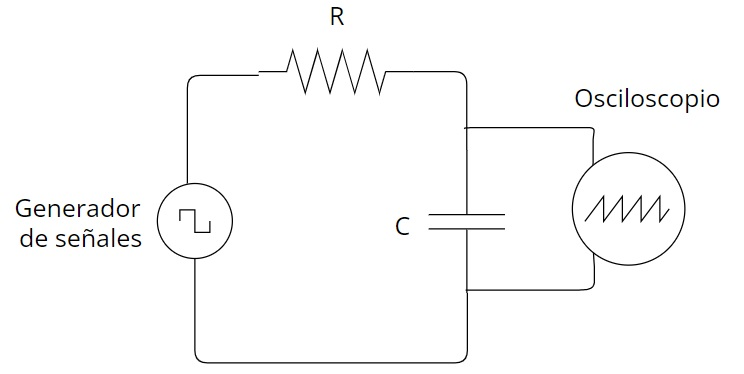
\includegraphics[width=0.4\linewidth]{CircuitoRC3.jpg}
    \caption{Esquema del Circuito utilizado}
\end{figure}
    El generador se mantuvo a una frecuencia aproximadamente de $Hz$, pero se llegaba a variar unos $100$. Para hacer las mediciones, se observó en el osciloscopio la caída de la descarga en el capacitor. Por un lado, en el eje y se tiene el voltaje asociado al capacitor, y en el eje x tenemos el tiempo en el que se va dando la descarga. La medición depende de la escala que se tenga en el osciloscopio.

    Los pares de Resistencia-capacitores fueron los siguientes: ($4.7k\Omega - 1\mu F$), \\ ($1.6k\Omega - 1\mu F$), ($1.6k\Omega - 1nF$), ($1.6k\Omega - 12.0nF$), ($0.1k\Omega - 12nF$).
\section{Resultados y discusión}
\subsection{Resistencias en paralelo y en serie}
\subsubsection{Arreglo en serie}
Para las resistencias iguales obtuvimos lo siguiente en 'Cuadro 1'.
\begin{table}[h]
\centering
\begin{tabular}{|l|r|r|}
\hline
     & \multicolumn{1}{l|}{Teórico} & \multicolumn{1}{l|}{Experimental} \\ \hline
$i_1 & 0.017                & 0.025                             \\ \hline
$i_2$ & 0.017                & 0.025                             \\ \hline
$i_3$ & 0.017                & 0.025                             \\ \hline
$i_T$ & 0.017                & 0.025                             \\ \hline
$R_1$ & 99.5                         & 99.5                              \\ \hline
$R_2$ & 99.5                         & 99.5                              \\ \hline
$R_3$ & 99.5                         & 99.5                              \\ \hline
$R_T$ & 298.5                        & 298.9                             \\ \hline
$V_1$ & 1.666                  & 1.665                             \\ \hline
$V_2$ & 1.666                  & 1.666                             \\ \hline
$V_3$ & 1.666                  & 1.666                             \\ \hline
$V_T$ & 5                            & 4.96                              \\ \hline
\end{tabular}
\caption{Tabla sobre la intensidad de corriente $\pm 0.0005$(A), resistencia $\pm 0.05$ ($\Omega$), voltaje $\pm 0.0005$ (V) del arreglo en serie (caso de resistencias iguales) siendo comparado con los datos teóricos}
\end{table}
Es destacable mencionar que la resistencia individual se consideró igual en la teoría como en la experimental, pues en la práctica la leyenda en el código de colores que expresa la resistencia es mucho más imprecisa que la leída en el multímetro, sin embargo sí hemos tomado el valor de 5V fijo en el voltaje total ya que es el expresado por la fuente de poder verificado con el multímetro (y el experimento planteaba este voltaje fijo); nótese que la intensidad de corriente a pesar de medirse desde los extremos de cada resistencia en comparación de la medida al rastrear desde la patita de la primera resistencia hasta la patita opuesta de la última se mantiene exactamente igual, la teoría nos indica un valor de 0.017A en contraste con ($0.025 \pm 0.0005$), que si bien discrepa ligeramente y se sale del intervalo de incertidumbre, se sigue manteniendo en el mismo orden de magnitud, asociamos esta discrepancia con el valor real que sienten las resistencias al evaluar su circulación de voltaje pues es distinto a 5V. Las resistencias al ser evaluadas en serie nos dieron un valor muy ligeramente mayor al de la teoría, esto debe ser porque existe cierta resistencia en las varillas conductoras del protoboard pues no son conductores perfectos. El voltaje total finalmente observamos que es levemente menor el experimental que el teórico, nuevamente lo asociamos a la conductividad del protoboard así como de los cables que están sujetos por un caimán en un estado no muy ideal que pudo interferir.\\

\begin{table}[h]
\centering
\begin{tabular}{|l|r|r|}
\hline
     & \multicolumn{1}{l|}{teórico} & \multicolumn{1}{l|}{experimental} \\ \hline
$i_1$ & 0.010                & 0.013                             \\ \hline
$i_2$ & 0.010                & 0.012                             \\ \hline
$i_3$ & 0.011                & 0.011                             \\ \hline
$i_T$ & 0.010                & 0.012                             \\ \hline
$R_1$ & 99.5                         & 99.5                              \\ \hline
$R_2$ & 330.7                        & 330.7                             \\ \hline
$R_3$ & 56.3                         & 56.3                              \\ \hline
$R_T$ & 486.5                        & 488.2                             \\ \hline
$V_1$ & 1.024                        & 1.005                             \\ \hline
$V_2$ & 3.405                        & 3.397                             \\ \hline
$V_3$ & 0.587                        & 0.592                             \\ \hline
$V_T$ & 5.0                         & 5.002                             \\ \hline
\end{tabular}
\caption{Tabla sobre la intensidad de corriente $\pm 0.0005$(A), resistencia $\pm 0.05$ ($\Omega$), voltaje $\pm 0.0005$ (V) del arreglo en serie (caso de resistencias diferentes) siendo comparado con los datos teóricos}
\end{table}

Para las resistencias diferentes se presenta la tabla ('Cuadro 2'), aquí el amperaje experimental se ha comportado ligeramente mayor que el teórico pero con una diferencia de ($0.003 \pm 0.0005$)A, quien es bastante despreciable, para los valores del voltaje han tendido a bajar los valores obtenidos experimentalmente que el teórico, en este caso es dificil decir si esto puede estar asociado a la resistencia del material conductor del protoboard, pues en un valor incrementó en contraste a lo teórico y en el total inclusive aparece un voltaje mayor que el reportado por la fuente.\\\\

Hemos visto entonces que es correcto la convención de aplicar una suma directa en las resistencias cuando están en serie, que la corriente se mantiene igual y que el voltaje es la suma de los voltajes individuales en cada resistencia.

\subsubsection{Arreglo en paralelo}
Para las resistencias iguales se obtuvo lo siguiente.

\begin{table}[h]
\centering
\begin{tabular}{|l|r|r|}
\hline
     & \multicolumn{1}{l|}{teórico} & \multicolumn{1}{l|}{experimental} \\ \hline
$i_1$ & 0.151                        & 0.209                             \\ \hline
$i_2$ & 0.151                        & 0.209                             \\ \hline
$i_3$ & 0.151                        & 0.209                             \\ \hline
$i_T$ & 0.452                        & 0.62                              \\ \hline
$R_1$ & 99.5                         & 99.5                              \\ \hline
$R_2$ & 99.5                         & 99.5                              \\ \hline
$R_3$ & 99.5                         & 99.5                              \\ \hline
$R_T$ & 33.17                  & 33.2                              \\ \hline
$V_1$ & 5                            & 5                                 \\ \hline
$V_2$ & 5                            & 5                                 \\ \hline
$V_3$ & 5                            & 5                                 \\ \hline
$V_T$ & 5                            & 5                                 \\ \hline
\end{tabular}
\caption{Tabla sobre la intensidad de corriente $\pm 0.0005$(A), resistencia $\pm 0.05$ ($\Omega$), voltaje $\pm 0.0005$ (V) del arreglo en paralelo (caso de resistencias iguales) siendo comparado con los datos teóricos}
\end{table}

Notamos que la corriente reportada experimentalmente es mayor que la teórica por una cantidad notable $(0.058 \pm 0.0005)A$, pero el valor es totalmente consistente para cada resistencia, lo preocupante es el amperaje total que muestra una diferencia importante, aunque al ver los datos de intensidad de corriente podemos ver que la regla de $A_T = \sum A_i$ se cumple por lo que la ley se cumple pero los datos de corriente eléctrica son distintos a la teoría por factores externos. Para la resistencia observamos datos casi totalmente idénticos a la teoría y en el voltaje son totalmente iguales.
\newpage
Para las resistencias distintas obtenemos lo siguiente.
\begin{table}[h]
\centering
\begin{tabular}{|l|r|r|}
\hline
     & \multicolumn{1}{l|}{teórico} & \multicolumn{1}{l|}{experimental} \\ \hline
$i_1$ & 0.22                         & 0.221                             \\ \hline
$i_2$ & 0.22                         & 0.220                              \\ \hline
$i_3$ & 0.22                         & 0.223                             \\ \hline
$i_T$ & 0.66                         & 0.662                             \\ \hline
$R_1$ & 99.5                         & 99.5                              \\ \hline
$R_2$ & 330.7                        & 330.7                             \\ \hline
$R_3$ & 56.3                         & 56.3                              \\ \hline
$R_T$ & 486.5                        & 487.1                             \\ \hline
$V_1$ & 5                            & 4.93                              \\ \hline
$V_2$ & 5                            & 5                                 \\ \hline
$V_3$ & 5                            & 4.95                              \\ \hline
$V_T$ & 5                            & 4.95                              \\ \hline
\end{tabular}
\caption{Tabla sobre la intensidad de corriente $\pm 0.0005$(A), resistencia $\pm 0.05$ ($\Omega$), voltaje $\pm 0.0005$ (V) del arreglo en paralelo (caso de resistencias diferentes) siendo comparado con los datos teóricos}
\end{table}

Notamos que la intensidad de corriente experimental es muy fiel a la teórica, a pesar de que en primera instancia hemos tenido un error pues se pensaría que la corriente sería distinta en cada resistencia justo por esto (por su resistencia), pero el experimento nos a arrojado datos muy consistentes. Aunque es probable que hayamos tenido un error en nuestra forma de obtener el muestreo de los amperajes y por ello esta relación extraña; el voltaje a pesar de fluctuar, esto es por las incertidumbres asociadas a los aparatos de medición a pesar de variaciones debido a factores de imperfección de los componentes, por lo que podemos decir que es el mismo para cada resistencia asímismo para la total, algo esperable pues se encuentran en la misma diferencia de potencial.

Hemos visto entonces que es verdad la ley que establece el inverso de una resistencia equivalente igual a la suma de los inversos de cada resistencia en el caso de resistencias paralelas, así como la intensidad de corriente total es la suma de las contribuciones iguales y que todas se encuentran a la misma caída de potencial.

\subsection{Descarga del capacitor.}

\subsubsection{Resistencia de $1.6k\Omega$ y frecuencia digital de 280hz en el generador de señales}

Debido a la ambigüedad para obtener la constante temporal $\tau$ capturando imágenes, hemos decidido sacarla directamente observando el osciloscopio para guiarnos con las cuadrículas que genera, sin embargo adjunto una imagen de uno de los gráficos donde explicaré lo que hemos hecho para cada uno de las combinaciones capacitor-resistencia.

\begin{figure}[h]
    \centering
    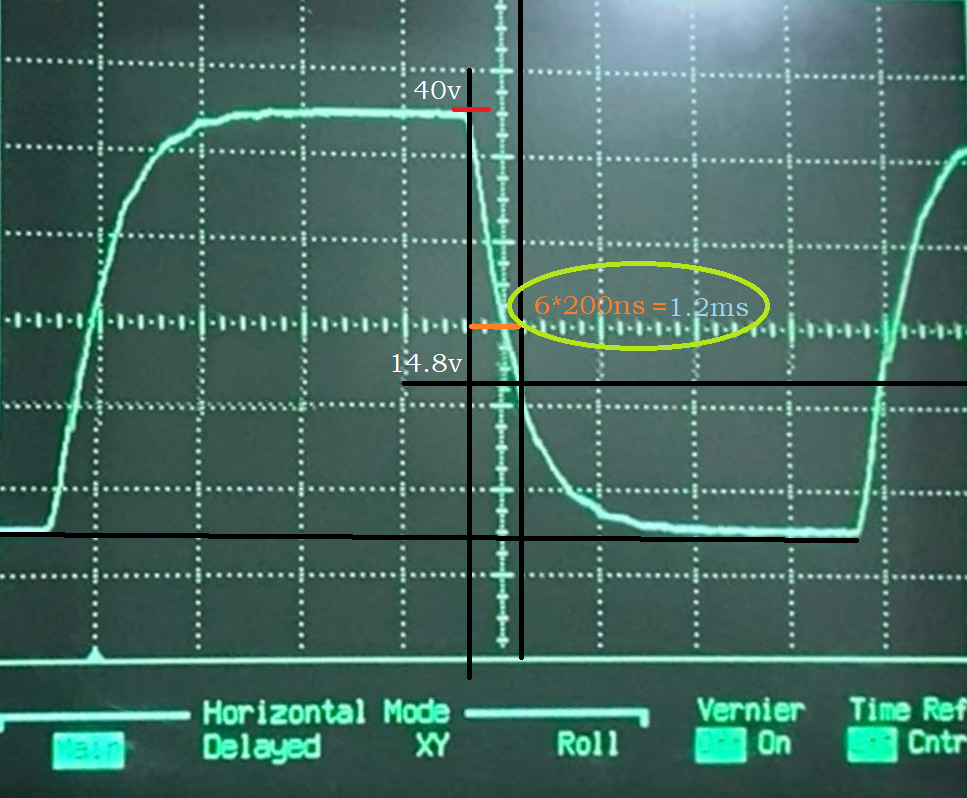
\includegraphics[width=1\linewidth]{image.png}
    \caption{Gráfica V(t) vs t de la pareja capacitor de $1 \mu F$ y resistencia de $1 k\Omega$. La cuadrícula mínima en y indica 2V mientras que la cuadrícula mínima en x indica 200ns}
    \label{fig:enter-label}
\end{figure}

Nótese que el voltaje en el que se carga totalmente son 40V, pues es la diferencia entre el punto más alto y más bajo en el gráfico, este valor fue multiplicado por 0.37 pues la teoría nos dice que en la fase de descarga, al llegar a $0.37V_0$ tal que $V_0$ es la carga máxima, nos indica que el tiempo transcurrido en este momento es tau. Por lo que trazamos una línea vertical en el punto $V_0=40V$ y otra en $0.37V_0=14.8V$, finalmente vemos el tiempo transcurrido entre estos dos valores el cual fue de 6 rayas, cada una representando 200ns y de aquí se sabe que tau es $\tau = 1.2ms$. Lo cual es muy cercano a lo que nos dice la teoría pues $\tau = RC = 1.6 \cdot 10^3 \cdot 1 \cdot 10^{-6} s = 1.6 ms$. Nótese que la incertidumbre asociada para cada tau es la asociada al producto RC, quien es $2.5\%$ del valor final.

Para la siguiente combinación con un capacitor de $1nF$ obtuvimos mediante el mismo análisis que la constante tau es de $1.0ps$, esto es más bajo de lo esperado pues la teoría nos indica un valor de $1.6ps$; finalmente para la combinación con un capacitor de 12nF el resultado es demasiado extraño, nos replicó el tiempo tau del primer capacitor $\tau = 1.2ms$, de hecho la imagen se ve completamente igual a la de este capacitor, la teoría nos indica que debería ser $19.2pF$, creímos que el error se debió al haber malinterpretado las unidades de medidas pues el capacitor citaba ser de $12.000pF$, sin embargo la conversión efectivamente fueron $12nF$ por lo que en vista de que no nos fueron proporcionados capacitómetros, sugerimos para un siguiente estudie se observe la verdadera capacitancia de este; para estas primeras mediciones se nos hace extraño que la tau sea mayor a lo que debería ser, esto nos dice que ya sea la capacitancia o la resistencia son menor a la reportada, nos inclinamos más hacia el caso que la capacitancia sea menor.

\subsubsection{Resistencia de $4.7k\Omega$ y frecuencia digital de 590hz en el generador de señales}
Para nuestra primera configuración con un capacitor de $1\mu F$, la tau experimental que observamos fue $5.4ms$, pero la teoría nos indica que debe ser de $4.7ms$, es curioso ver que aquí es mayor que la teoría, por lo que nos inclinamos ahora a que el factor que aumenta nuestro RC es la resistencia, ya que hemos tenido que cambiar de protoboard después del dato tan extraño que se obtuvo en la medición de la última tao para la resistencia de $1.6 k\Omega$, debemos recordar esto pues lo esperado es que desde esta medición en adelante nuestros taus experimentales excedan a lo mostrado en la teoría si nuestra hipótesis es cierta.
Para la segunda combinación con 12nF nuestra constante tau es de $0.4ms$, esto está muy errado pues la teoría indica que debe ser $\tau = 56.4pF$.
A partir de esta medición las demás estuvieron peor, hemos intentado combinaciones que ya habían funcionado antes pero no hemos tenido éxito en visualizar sus curvas, se nos fue comentado que existe una alta probabilidad que sea a causa del calentamiento del generador de señales, por lo cual esta segunda medición para esta resistencia no nos parece fiel al fenómeno y la descartaremos así como la tercera de la primer resistencia. Debido a este calentamiento del generador de señales, ya no hubo una tercera combinación RC para esta resistencia ya que los resultados no eran replicables.


\section{Conclusiones}

En este estudio, hemos analizado y verificado experimentalmente principios fundamentales relacionados con circuitos resistivos y capacitivos, incluyendo configuraciones en serie y en paralelo de resistencias, así como la dinámica de carga y descarga de un circuito RC. La investigación ha resaltado varios aspectos clave de los circuitos eléctricos y ha corroborado leyes teóricas, como las Leyes de Kirchhoff y la Ley de Ohm, en aplicaciones prácticas.

En cuanto a redes resistivas, se exploraron tanto configuraciones en serie como en paralelo. En la configuración en serie, los datos experimentales coincidieron estrechamente con las expectativas teóricas, demostrando que la resistencia total es la suma de las resistencias individuales, mientras que la corriente permanece constante en cada resistencia. Las caídas de voltaje observadas en las resistencias individuales sumaron el voltaje total aplicado, validando la Ley de Voltajes de Kirchhoff en circuitos en serie. Las discrepancias observadas en las mediciones experimentales fueron mínimas y probablemente atribuibles a pérdidas resistivas en los conductores de conexión y a la resistencia inherente de los contactos de la protoboard. En cuanto a resistencias en paralelo, los resultados experimentales nuevamente se alinearon bien con las predicciones teóricas. En este caso, se observó que la resistencia total disminuye a medida que se agregan más resistencias en paralelo, confirmando que la resistencia general en un circuito paralelo es inversamente proporcional a la suma de las conductancias individuales. La corriente a través de cada resistencia varió en función de su resistencia, cumpliendo con la Ley de Corrientes de Kirchhoff, mientras que el voltaje en cada resistencia fue consistente con el voltaje de la fuente aplicada.

Al examinar los circuitos RC, el enfoque se centró en el comportamiento de carga y descarga del capacitor. El tiempo constante \(\tau\) se determinó experimentalmente como el producto de la resistencia y la capacitancia, proporcionando una medida de la rapidez con que el capacitor se carga o descarga. Al observar la curva de descarga del capacitor, que mostró una disminución exponencial, pudimos identificar empíricamente \(\tau\) como el punto en el que la carga del capacitor alcanzó aproximadamente el 36.8\% de su valor inicial. Este comportamiento coincide con el modelo teórico para un circuito RC, donde la tasa de descarga depende exponencialmente del tiempo constante. Los resultados experimentales mostraron ligeras variaciones respecto a las predicciones teóricas, debido principalmente a limitaciones prácticas como la precisión del osciloscopio y la exactitud de los valores de los componentes.

\newpage
\noindent {\bf Declaración de contribución de los autores}\\ 

Iván Bautista Alvarado$^1$ y Andrés López González$^1$ hemos realizado tanto el apartado escrito como el análisis de manera colectiva siendo una participación del 100\% por parte de ambos y no solo una repartición.\\ 

{\bf Agradecimientos} \\ 

A ese.\\

\begin{figure}[h]
    \centering
    
\includegraphics[width=0.5\linewidth]{el.png}
    \caption{Electrogato}
    \label{fig:enter-label}
\end{figure}\\

\begin{thebibliography}{99}

\bibitem{griffiths}
D. J. Griffiths, \textit{Introduction to Electrodynamics}, 3rd ed. Upper Saddle River, NJ, USA: Prentice-Hall, 1999.

\bibitem{jackson}
J. D. Jackson, \textit{Classical Electrodynamics}, 3rd ed. New York, NY, USA: Wiley, 1998.

\bibitem{sadiku}
M. N. O. Sadiku, \textit{Elements of Electromagnetics}, 6th ed. New York, NY, USA: Oxford University Press, 2014.

\bibitem{wangsness}
R. K. Wangsness, \textit{Electromagnetic Fields}, 2nd ed. New York, NY, USA: Wiley, 1986.

\bibitem{zangwill}
A. Zangwill, \textit{Modern Electrodynamics}. Cambridge, UK: Cambridge University Press, 2013.

\bibitem{purcell}
E. M. Purcell and D. J. Morin, \textit{Electricity and Magnetism}, 3rd ed. Cambridge, UK: Cambridge University Press, 2013.

\bibitem{shadowitz}
A. Shadowitz, \textit{The Electromagnetic Field}. Mineola, NY, USA: Dover Publications, 1988.


\end{thebibliography}


\end{document}

